\documentclass[12pt]{article}
\usepackage[a4paper, total={6in, 8in}]{geometry}
\usepackage{extsizes}
\renewcommand{\baselinestretch}{1.5}

\usepackage{fontspec}
\setmainfont{Times New Roman}

\usepackage[BoldFont, SlantFont]{xeCJK}
\setCJKmainfont{BiauKai}

\usepackage{amsmath,amssymb}
\usepackage[title]{appendix}
\usepackage{fullpage,graphicx,listings,xcolor,booktabs,pgfplots}
\usepackage[hidelinks]{hyperref}
\usepackage[small,bf]{caption}
\usepackage{subcaption}
\setlength{\abovecaptionskip}{2pt plus 2pt minus 2pt}
\usetikzlibrary{intersections}

\definecolor{bgcolor}{rgb}{0.95,0.95,0.95}
\lstdefinestyle{mystyle}{
basicstyle=\footnotesize\ttfamily,
backgroundcolor=\color{bgcolor},
keywordstyle=\color{violet},
stringstyle=\color{red},
commentstyle=\color{gray},
showstringspaces=false,
numbers=left,
frame=line
}
\lstset{
style=mystyle,
breaklines=true,
postbreak=\mbox{\textcolor{red}{$\hookrightarrow$}\space}
}

\bibliographystyle{acm}

\begin{document}
\begin{titlepage}
\begin{center}
\vspace*{2cm}
{\bf \LARGE TSM-Net: 以對抗式時序壓縮自編碼器為基礎的\\音訊變速演算法} \\
\vspace*{0.3cm}
{\bf \LARGE TSM-Net: Temporal Compressing Autoencoder with Adversarial Losses for Time-Scale Modification on Audio Signals} \\[2cm]
{\large 國立中山大學資訊工程學系} \\
{\large 110 學年度大學部專題製作競賽} \\[2cm]
{\large 組員:B073040018 朱劭璿} \\
{\large \hspace{1.55cm}B072010029 陳居廷} \\[2cm]
{\large 指導教師:陳嘉平 教授}
\end{center}
\end{titlepage}
\newpage
\begin{abstract}
We proposed a novel approach in the field of time-scale modification on the audio signals. While traditional methods use framing technique and spectral approaches use short-time Fourier transform to get high-level units. TSM-Net, our neural-network model encodes the raw audio into a high-level latent representation called Neuralgram. Since the resulting Neuralgram is a two-dimensional image with real values, we apply some existing image resizing techniques on the Neuralgram and decode it using our neural decoder to obtain the time-scaled audio. Our method yields little artifacts and opens a new possibility in the research of modern time-scale modification.
\end{abstract}
\newpage
\tableofcontents
\newpage

\section{Introduction}
With the advance of technologies and digitalization, we can store and reproduce multimedia content nowadays. We can even manipulate the materials in a way that we couldn't imagine before digitalization. For example, image resizing and video editing, which change the dimensionality of the digital pictures spatially and temporally, respectively. Another ubiquitous application regarding audio signals called time-scaled modification (TSM) is used in our daily life. It's also known as playback speed control in the video streaming platforms such as YouTube.

With the power of artificial intelligence (AI) and modern computation hardware, however, we haven't discovered any method using AI to refine TSM algorithm and leverage the quality of the synthetic audio to the next level. Consider we have pragmatic AI tools in similar domains like image super-resolution \cite{led17} and motion estimation and motion compensation (MEMC) \cite{bao21}, etc.

\subsection{Time-scale modification}
\paragraph{Time-domain approach}
The main idea of TSM is that instead of scaling the raw waveforms on the time axis, which leads to pitch shifts due to the changes of wavelengths, we segment the audio into small chunks of fixed length, a.k.a frames or windows to keep the wavelength intact. In order to minimize the boundary breakage after processing, the adjacent frames are overlapped and rearranged to obtain the synthetic audio. As shown in Figure \ref{fig:tsm-pipeline}. The original distance between the start of each frame is called analysis hop size. After frame relocation, the distance becomes synthesis hop size, and the ratio of the analysis hop size and the synthesis hop size is the rate at which the audio is sped up or down \cite{dri16}. In addition, the Hann window \cite{ess86} is applied to each analysis frame to maintain the amplitude of overlapped areas. The main challenge is the harmonic alignment problem, as shown in Figure \ref{fig:harmonic-alignment}. With significant periodicities, an unconstrained ratio of the analysis to synthesis hop size can cause a discrepancy with the original waveform. Specifically, the phases of the same frequency components in the frames do not synchronize properly, which leads to serious interference despite the identical waveforms. Several enhancements have been proposed to solve the synchronization problem \cite{hej91}\cite{eri90}\cite{ver93}. However, the resultant sound is usually non-natural and contains audible clipping artifacts. This is the negative effect of the framing technique. Moreover, the time-domain TSM only preserves the most prominent periodicity. For the audio with a wide range of frequencies composition, like pop music, symphony and orchestra, the less prominent sound are often erased in the process.

\begin{figure}
\begin{center}
  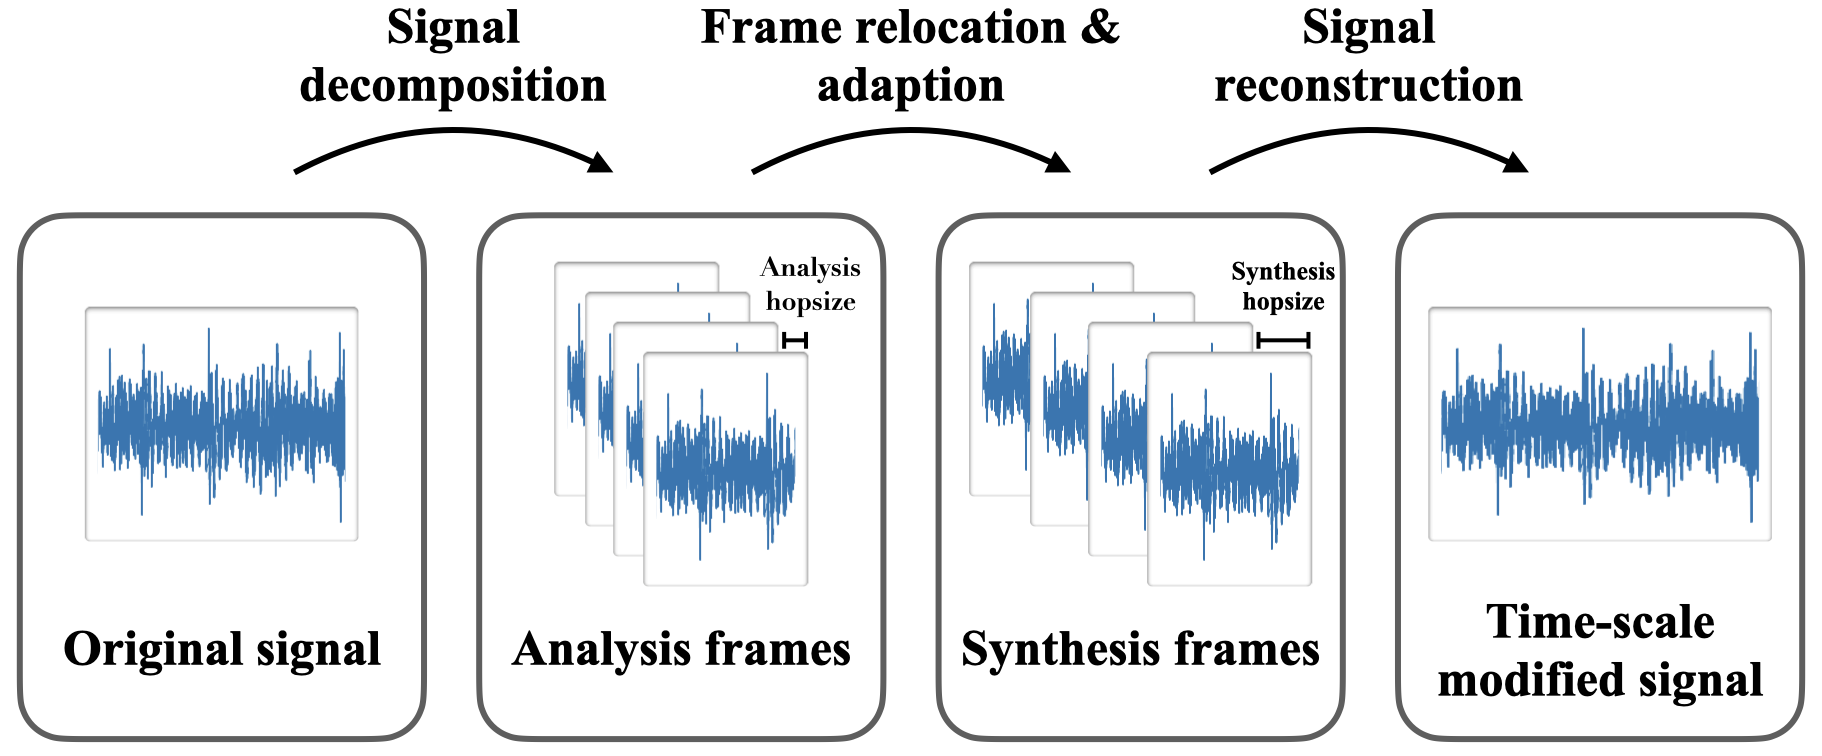
\includegraphics[width=.8\textwidth]{assets/figures/tsm-pipeline}
\end{center}
\caption{Generic processing pipeline of time-domain time-scale modification (TSM) procedures.}
\label{fig:tsm-pipeline}
\end{figure}

\begin{figure}
\begin{center}
  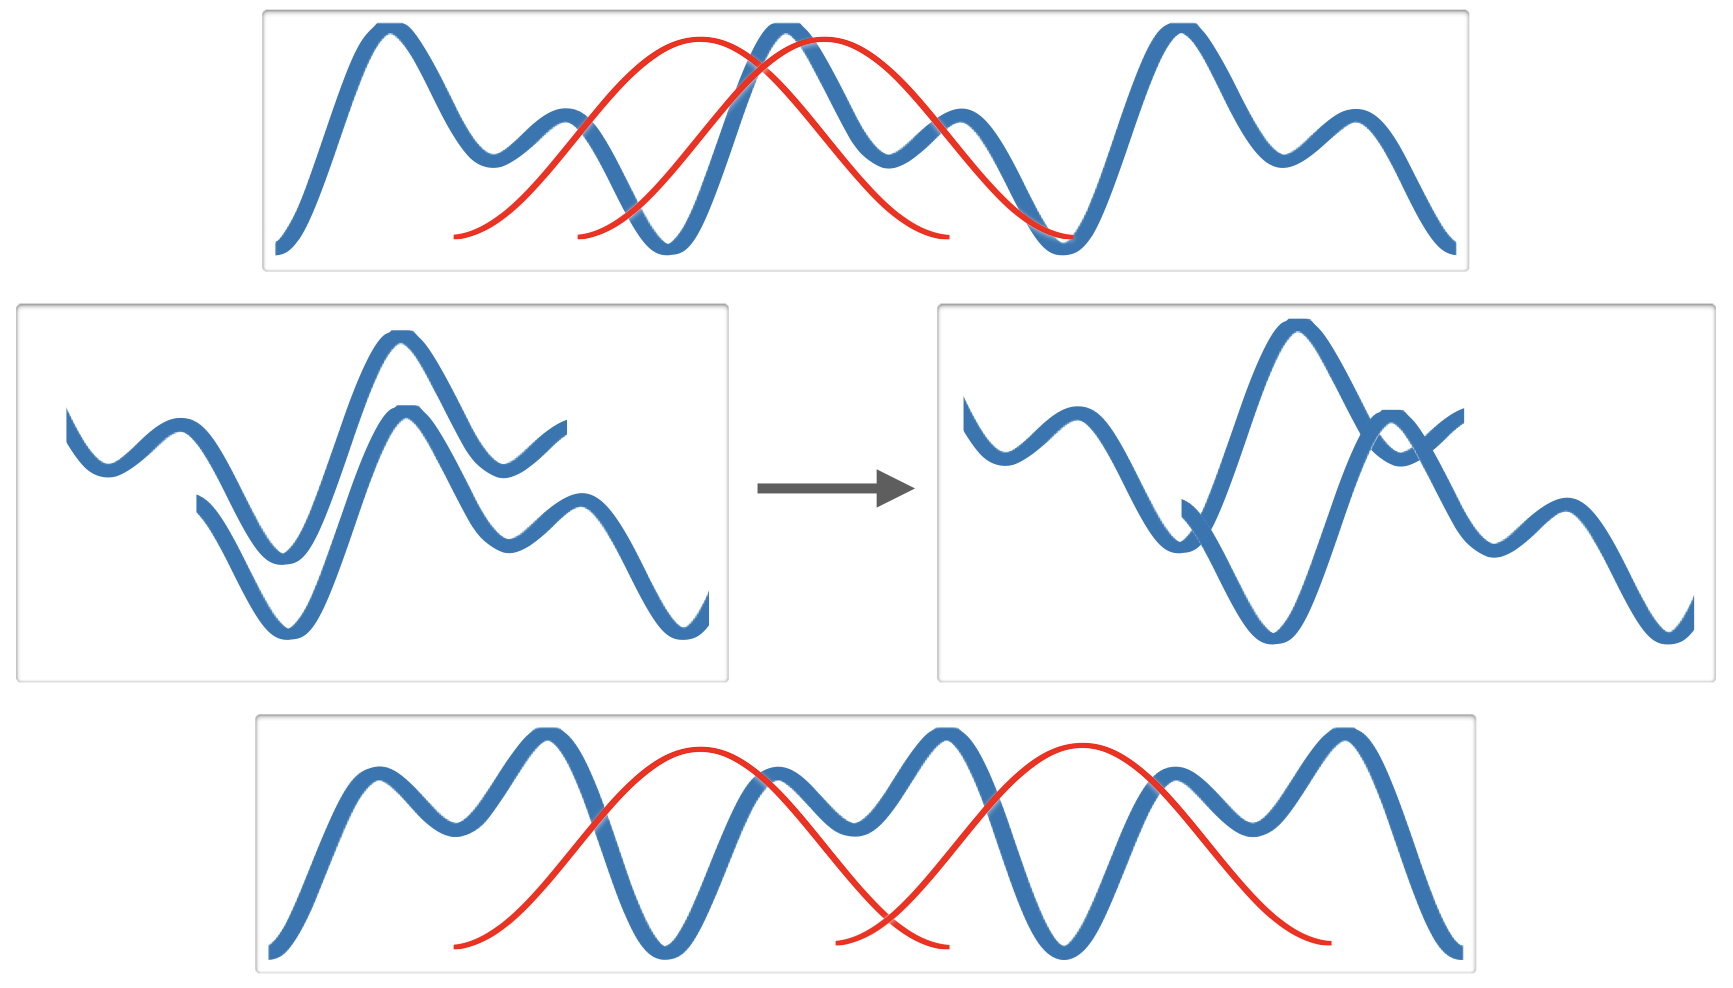
\includegraphics[width=0.8\textwidth]{assets/figures/harmonic-aligment}
\end{center}
\caption{An illustration of the harmonic alignment problem. The red Hann windows indicate the rearrangement of the frames. An unconstrained scale ratio would lead to serious interference.}
\label{fig:harmonic-alignment}
\end{figure}

\paragraph{Spectral-domain approach}
Another approach tries to manipulate the audio in the spectral space, using short-time Fourier transform (STFT) to convert the frequency information in the raw waveform to a more semantic representation with complex numbers \cite{lar99}. The magnitude and phase parts can be further derived. Unfortunately, unlike the magnitudes, which give constructive and straightforward audio features, the phases are relatively complicated and hard to model. Moreover, due to the heavy correlation between each phase bin, we have to use a phase vocoder \cite{fla66} to estimate phases and the instantaneous frequencies after carefully relocate STFT bins to avoid a peculiar artifacts, a.k.a. phasiness. Despite some refined methods \cite{kra12}\cite{moi11}\cite{nag09}, which improve both the vertical and horizontal phase coherence, the spectral representation is essentially not directly scalable, and the iterative phase propagation process in the phase vocoder is an inevitable overhead.

\subsection{Harnessing the power of neural networks}
As we've mentioned above, the task requires a highly temporally compressed representation of the audio signals. The neural networks naturally come into our minds. The neural networks are composed of a sequence of linear transformations joined by nonlinear activation functions. With numerous configurable parameters, also known as weights, they are capable of approximating almost any function we desire, including the compression function that transforms the raw audio waveforms into low-dimensional latent vectors and back. The parameters are initially random noises and can be gradually inferred using a technique called gradient descent, in which we specify a meaningful loss function such as the difference between the networks' output and the target value, then the parameters can be configured based on the gradients of the loss function so the output would slowly move toward the target value.

\paragraph{TSM-Net}
To transform back and forth in two domains, we can think of the neural networks as an encoder and a decoder, in the jargon of machine learning, this kind of architecture is called autoencoder \cite{kra91}, which encodes the data into a high-level (and typically low-dimensional) latent vectors and tries its best to decode it back to the original data. In our neural network model, the dimension of the latent vectors is 1024 times smaller than the original one, which means one sample in the latent vector can represent more than an entire wave in the raw audio waveform. Since the latent vector is an image-like multi-dimension vector, we can apply the existing image resizing techniques to scale it. Finally, we decode the resized latent vector to obtain the time-scaled audio waveform.

\paragraph{Distribution modeling}
In order to make the model generalizes on the unseen data, we have to model the data distribution instead of directly measuring the L2 distance on the existing dataset, which leads to blurry output upon unseen data. Therefore, we employ a discriminative neural network to help us train the autoencoder \cite{goo14}. The discriminative network computes the adversarial loss, which measures how well it distinguishes the real and generated data. We will go into detail about the training objective and its effectiveness later.

\section{Related Works}
Modeling audio is not a trivial task for neural networks. To illustrate it, we can take image generation for example. DCGAN \cite{rad16} is a generative neural network which synthesizes realistic images with dimension of $3\times 64\times 64$. There are 12288 pixels that the model needs to estimate. A 5 seconds stereo audio clip with sampling rate of 22050 Hz has $2\times 5 \times 22050 = 220500$ samples. Not to mention each pixel is stored in 8 bits while each audio sample is stored in 16 bits and has 256 times possible values than an image pixel. Decreasing the sampling rate to simplify the dimensionality is another option. However, the Nyquist-Shannon sampling theorem suggests that the low sampling rate would lead to serious aliasing.

\subsection{Neural vocoder} Models that directly generate raw audio waveform are known as vocoder. A vocoder can be conditioned on some high-level abstract features such as linguistic features or spectrograms. The spectrogram is the magnitude part from the output of STFT. It expresses the frequency composition clearly and is easy to model thanks to its smooth variations over time. As mentioned above, the phases are relative hard to estimate, therefore in applications like text-to-speech (TTS) \cite{xu21} pipeline, the network often predicts the speech spectrogram of given texts, then uses a vocoder to get the raw audio. The early vocoders include Griffin-Lim \cite{gri84}, WORLD \cite{mor16}, etc. The modern neural-based vocoders start with WaveNet \cite{aar16}, which predicts the distribution for each audio sample conditioned on all previous ones. However, the autoregressive model runs too slow to apply on real-time applications. FloWaveNet \cite{sun18} and WaveGlow \cite{pre19} are neural vocoders based on bipartite transforms. They present a faster inference speed and high-quality synthetic audio but require larger models and more parameters to be as expressive as the autoregressive models, and thus harder to train. WaveGAN \cite{chr18}, MelGAN \cite{kun19} and VocGAN \cite{yan20} employ the generative adversarial network \cite{goo14} training architecture in which a discriminator is used to measure the divergence of synthetic audio and the real audio and try to learn the generator optimal weights to make the synthetic audio as realistic as possible. The discriminator usually works in multiple scales in order to take care of different frequency bands in the audio data. This kind of approach allows small models to generate high-fidelity audio samples.

\subsection{Nyquist-Shannon sampling theorem} The sampling rate is the number of samples per second that a signal is recorded, and the bit depth is the amplitude precision in which each sample is stored. The analog continuous signal has to be discretized and quantized in order to be stored digitally in the computer. Specifically, discretization and quantization transfer continuous signals into discrete counterparts along the time and amplitude axis, respectively. Common combinations include 44100Hz/24bit, 22050Hz/16bit, 16000Hz/16bit, etc. A lower sampling rate results in lower data dimension, which is beneficial for reducing modeling complexity. However, a lower sampling rate is easier to produce aliasing. Aliasing is a phenomenon where two different signals alias one another in the discrete domain as illustrated in Figure \ref{fig:3}. As pointed out and proven by Nyquist \cite{nyq28} and Shannon \cite{sha48}, a signal containing no frequency higher or equal than $\omega$Hz, is completely determined by sampling at $2\omega$Hz, i.e., to resolve all frequencies in a signal, it has to be sampled at strictly greater than twice the highest frequency present. Otherwise, the discrete representation cannot determine some high-frequency components which have low-frequency aliases. Aliasing sometimes happens in the real world where some human sensory organs have preceptive limitations. For example, human eyes can only see about 30 to 60 frames per second. For cars driven at a very high speed, the wheels spin too fast to be correctly perceived by human eyes, as if they're spinning backward. This is known as the wagon-wheel effect. Another example is the moiré pattern \cite{dan62}. It can be usually observed in the photographs of digital monitors. The resolution of the camera is not high enough to capture the pixels on the monitors and leads to artificial patterns.

\begin{figure}
\begin{center}

\begin{tikzpicture}
\begin{axis}[
  domain=0:10,
  axis lines = left,
  legend pos=outer north east,
  xlabel = \(x\),
  ylabel = {\(f(x)\)},
  width=8cm,
  height=2cm,
  scale only axis,
]
\addplot [
  name path=p1,
  samples=100, 
  color=red,
]
{sin(deg(x))};
\addlegendentry{$\sin(x)$}
\addplot [
  name path=p2,
  samples=100, 
  color=blue,
]
{sin(deg(2*x))};
\addlegendentry{$\sin(2x)$}

\fill 
  [name intersections={of=p1 and p2, name=i, total=\t}] 
  [black, opacity=1] 
  \foreach \s in {1,...,\t}{(i-\s) circle (2pt)};

\end{axis}
\end{tikzpicture}

\end{center}
\caption{An illustration for aliasing. Suppose the signals are sampled non-uniformly for better illustration, two signals with different frequency components are the aliases for each other in the discrete domain, represented as black dots.}
\label{fig:3}
\end{figure}

\section{Methodology}

\subsection{Latent representation}
We proposed a new representation for audio called Neuralgram to provide a novel approach to TSM. The Neuralgram is a temporally compressed feature map extracted from the middle of a neural autoencoder. A Neuralgram is applicable on TSM only when the following exists.
\begin{enumerate}
  \item{An encoder-decoder pair that is capable of fairly reconstructing the raw waveform.}
  \item{A compression ratio that is high enough to put an entire sinusoid of the lowest frequency present into one sample in the Neuralgram}
\end{enumerate}

Instead of directly scaling on the raw waveform, which leads to the pitch shifting, we encode the raw waveform as a real-valued Neuralgram and scale the Neuralgram. Finally, we decode the scaled Neuralgram to get time-scaled audio without pitch shifting, as illustrated in Figure \ref{fig:4}. Because one sample in neuralgram encodes more than an entire sinusoid for each frequency component, resizing the Neuralgram using Bilinear \cite{smi81} or Bicubic \cite{key81} interpolation can repeat the entire sinusoids in the reconstructed waveform rather than changing their wavelengths and frequencies.

\begin{figure}
\begin{center}
\begin{tabular}{l}
(a)
\begin{tikzpicture}
\begin{axis}[
  domain=0:3.14,
  axis lines = left,
  legend pos=outer north east,
  width=4cm,
  height=2cm,
  scale only axis,
]
\addplot [
  samples=100, 
  color=red,
]
{sin(deg(2*x))};

\end{axis}
\end{tikzpicture}

(b)
\begin{tikzpicture}
\begin{axis}[
  domain=0:6.28,
  axis lines = left,
  legend pos=outer north east,
  width=8cm,
  height=2cm,
  scale only axis,
]
\addplot [
  samples=100, 
  color=red,
]
{sin(deg(x))};

\end{axis}
\end{tikzpicture} \\

(c)
\begin{tikzpicture}
\begin{axis}[
  domain=0:3.14,
  axis lines = left,
  legend pos=outer north east,
  width=4cm,
  height=2cm,
  scale only axis,
]
\addplot [
  samples=100, 
  color=blue,
]
{sin(deg(2*x))};

\end{axis}
\end{tikzpicture}

(d)
\begin{tikzpicture}
\begin{axis}[
  domain=0:6.28,
  axis lines = left,
  legend pos=outer north east,
  width=8cm,
  height=2cm,
  scale only axis,
]
\addplot [
  samples=100, 
  color=blue,
]
{sin(deg(2*x))};

\end{axis}
\end{tikzpicture}

\end{tabular}
\end{center}
\caption{An illustration for the desire TSM. The original signal contains the sinusoid for a single frequency (a,c). The erroneous signal (b) is the result of directly scaling on the raw waveform, which changes the wavelength of the sinusoid and produces pitch shifting. The desired behavior (d) can be achieved by scaling on the Neuralgram, which compresses the entire sinusoid into one sample.}
\label{fig:4}
\end{figure}

\paragraph{Neuralgram vs. Spectrogram}
In the literature, most of the works related to the neural vocoder use the spectrogram family as the modeling condition. Why do we bother to opt for a new representation? These traditional representations encode different frequency information into the same amount of samples in the latent space. This leads to different upsample scaling ratios during the decoding process depend on the frequency since each frequency has its own wavelength. Transformation function with the variable upsampling ratio is harder to approximate with convolutional generative models. On the other hand, our Neuralgram encodes different frequency components proportionally. This is intuitive for convolutional networks and the model is easier to train.

\subsection{The TSM-Net model}
\paragraph{Autoencoder}
Our model is adapted from the MelGAN \cite{kun19}. In the original generator, the input is a mel-spectrogram, which would be upsampled 256$\times$ to a raw audio waveform. In the proposed model, in order to compress the entire sinusoid into one sample, we increase the upsampling rate to 1024$\times$, because for audio with the sampling rate of 22050Hz, a 20Hz sinusoid, which is the lowest frequency the human ear perceives takes up 1102.5 samples. The upsampling is done in 5 stages of 8$\times$, 8$\times$, 4$\times$, 2$\times$ and 2$\times$ upsampling. In addition, we reverse the modified generator and prepend it to the front to obtain the full autoencoder model $A$. Both the encoder and the decoder are initiated by an aggregating convolutional layer then followed by each downsampling/upsampling stage. Each stage is composed of a dilated downsampling/upsampling convolutional layer and a residual block that also contains a dilated convolutional block and a skip-connection for the purpose of increasing receptive fields. As discussed in the MelGAN paper, we also use kernel-size as a multiple of stride in order to avoid checkerboard artifacts \cite{ode16} and weight normalization \cite{lee16} is also used after each layer to improve the sample quality. The full architecture of the autoencoder can be found in Table \ref{tab:arch-a-d}a.

\paragraph{Training objective}
We employ the same discriminators as the ones in the MelGAN. Three discriminators $(D_1, D_2, D_3)$ work in different scales simultaneously. Except for the one works in the original scale, $D_1$, the downsampling is performed beforehand using strided average pooling with kernel size 4. The architecture of each discriminator can be found in Table \ref{tab:arch-a-d}b. With such arrangements, it's easier to for each discriminator to learn features for different frequency range of the audio. We can now formulate the adversarial losses for training the autoencoder $A$. We follow the MelGAN and use the hinge loss version of the GAN objective \cite{lim17} to only penalize on the unstable data distribution. We also inherit the feature matching loss $mathcal{L}_{FM}$ additionally, which minimizes the L1 norm between the discriminator's feature maps of real and reconstructed audio. We accumulate the feature matching losses at each intermediate layer of all discriminator along with the training of the autoencoder.

\begin{equation}
  \mathcal{L}_{FM}\left( A, D_k\right) =
  \mathbb{E}_x\left[\sum_{i=1}^T \frac{1}{N_i}
  \lVert D_k^{(i)}(x) - D_k^{(i)}(A(s))\rVert_1
  \right]
\end{equation}

where $D_k^{(i)}$ represents the $i$th layer's feature map output of the $k$th discriminator. $N_i$ is a normalization factor and denotes the number of units in each layer. $T$ represents the number of layers in each discriminator. Our final training objective is shown as below with $\lambda = 10$.

\begin{equation}
\min_{D_k}\sum_{k=1}^3\mathbb{E}_x\left[
  \min\left( 0, 1 - D_k\left( x\right)\right) +
  \min\left( 0, 1 + D_k\left( A\left( x\right)\right)\right)
\right]
\end{equation}

\begin{equation}
\min_{A}\left(
  \mathbb{E}_x\left[-\sum_{k=1}^3D_k\left( A\left( x \right)\right)\right] +
  \lambda\sum_{k=1}^3\mathcal{L}_{FM}\left( A, D_k\right)
\right)
\end{equation}

where $x$ represents the raw audio waveform, $A$ represents the autoencoder, and $D_k$ represents each discriminator. According to \cite{mat16} and \cite{iso17}, the noise input is not necessary when the conditioning information is very strong in the generative model.

\section{Experiment}
We train our model with Tesla P100 on four Datasets, including FMA \cite{kir16}, Musicnet \cite{joh18}, VCTK \cite{yam19} and the audio from the Data Structure class recording \cite{chu21} lectured by Prof. C.B. Yang, NSYSU. All of the audio are resampled to 22050Hz. The audio samples can be found on our website\footnote{\url{https://dodoron241237.github.io/tsm-net-demo/}.}. We also use two additional metrics to monitor our training but they are not included in the training losses.
\begin{enumerate}
  \item{Audio Reconstruction (AR). AR is the L1 norm between the real and reconstructed raw audio waveform}
  \item{Neuralgram Reconstruction (NR). NR is the L1 norm between the Neuralgrams encoded from the real and reconstructed raw audio waveform, i.e., the reconstructed Neuralgram has 1.5 passes through the autoencoder.}
\end{enumerate}

\subsection{Training techniques}
The model is easy to train, taking around a weeks to train from scratch. However, it's not guaranteed to converge in every runs. A successfully converged run is shown in Figure \ref{fig:healthy-d}. A healthy loss for discriminator tend to fluctuate around 6. As long as the discriminator's loss decreases drastically, neither the autoencoder's loss nor the feature matching loss is able to return to a healthy value and diverges quickly, thus leading to poor quality. We can double check this phenomenon from the AR and NR. Both reconstruction losses increase after the discriminator dominates the training. We can also perceive notable background noises in the reconstructed audio samples.

\paragraph{Broken example} Sometimes, the model won't converge at all. As shown in Figure \ref{fig:broken-nr}, the NR loss becomes zero after 5 thousands iterations. Intuitively, no matter how good a model is, it's nearly impossible to have a loss of zero. Therefore in this case, the model is not optimized. On the contrary, the encoder discards the conditions and generates the same noisy Neuralgram regardless of the input. The reconstructed audio also only contains the same noise no matter what input is fed into the model. This failure mostly happens on the FMA dataset, which contains lots of Pop music. We suspect that the wide frequency range in the Pop music makes it more difficult to train from scratch. We try to pre-train the autoencoder or the discriminator on the Classical music dataset, Musicnet. A pre-trained autoencoder succeeds in making the discriminator's loss stable via transfer learning. On the contrary, a pre-trained discriminator cannot guide the autoencoder to perform proper reconstruction.

\begin{figure}
\begin{center}
  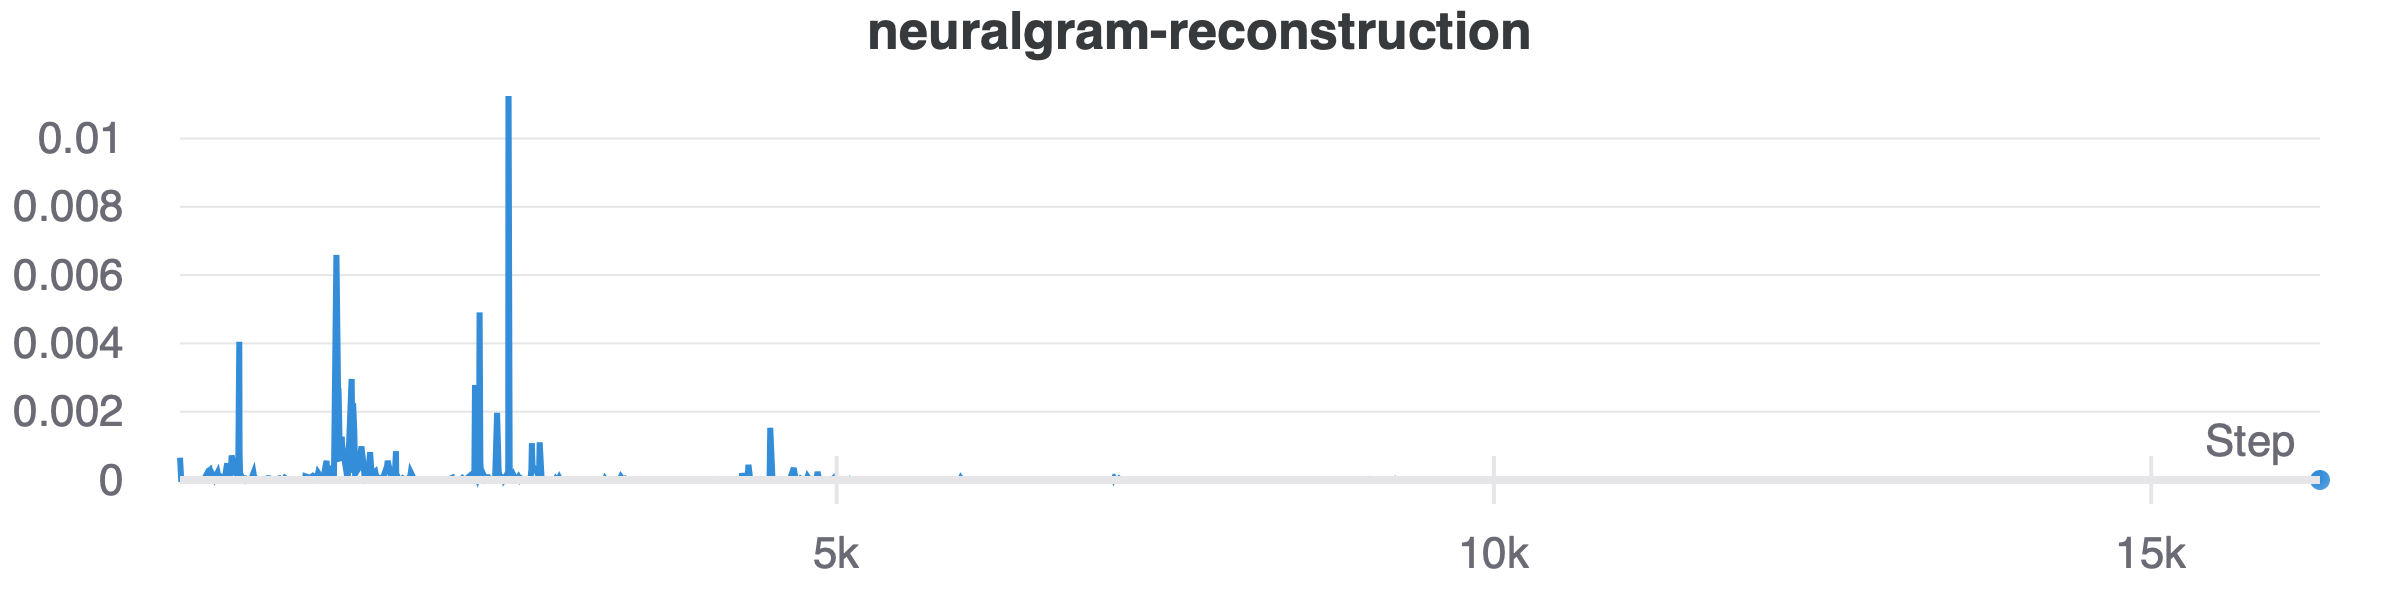
\includegraphics[width=\textwidth]{assets/figures/broken-nr}
\end{center}
\caption{A broken training run. The NR loss becomes zero after 5 thousands iterations.}
\label{fig:broken-nr}
\end{figure}

\subsection{Study on different compressing ratios}
As mentioned above, a compressing ratio (CR) of 1024$\times$ is large enough for the lowest perceivable frequency. We want to see whether a lower CR leads to the pitch shifting in TSM. We examine different models with CR of 256$\times$, 512$\times$ and the original 1024$\times$. Intuitively, the lower CR should provide smaller reconstruction errors, since the latent space is closer to the original data space. As expected, the pitch shifting gradually presents as the frequency goes down, and it seldom happens in the high frequencies. The smaller the CR, the higher frequency the pitch shifting spreads.

\section{Conclusion}


\bibliography{tsm-net}

\newpage
\renewcommand{\baselinestretch}{1}
\begin{appendices}
\section{Model Architecture}

\begin{table}[ht]
  \begin{subtable}{.49\linewidth}
  \centering{
    \begin{tabular}{c}
      \toprule
      \midrule
      Tanh 7 $\times$ 1, stride=1 conv 32 Tanh\\
      \midrule
      Residual Block 32\\
      \midrule
      Tanh 4 $\times$ 1, stride=2 conv 64 \\
      \midrule
      Residual Block 64\\
      \midrule
      Tanh 4 $\times$ 1, stride=2 conv 128 \\
      \midrule
      Residual Block 128\\
      \midrule
      Tanh 8 $\times$ 1, stride=4 conv 256 \\
      \midrule
      Residual Block 256\\
      \midrule
      Tanh 16 $\times$ 1, stride=8 conv 512\\
      \midrule
      Residual Block 512\\
      \midrule
      Tanh 16 $\times$ 1, stride=8 conv 1024\\
      \midrule
      Tanh 16 $\times$ 1, stride=8 conv transpose 512\\
      \midrule
      Residual Block 512\\
      \midrule
      Tanh 16 $\times$ 1, stride=8 conv transpose 256\\
      \midrule
      Residual Block 256\\
      \midrule
      Tanh 8 $\times$ 1, stride=4 conv transpose 128 \\
      \midrule
      Residual Block 128\\
      \midrule
      Tanh 4 $\times$ 1, stride=2 conv transpose 64 \\
      \midrule
      Residual Block 64\\
      \midrule
      Tanh 4 $\times$ 1, stride=2 conv transpose 32 \\
      \midrule
      Residual Block 32\\
      \midrule
      Tanh 7 $\times$ 1, stride=1 conv 1 Tanh\\
      \midrule
      \bottomrule
  \end{tabular}
  }
	\caption{Autoencoder architecture for TSM-Net }
  \end{subtable}
  \begin{subtable}{.49\linewidth}
  \centering{
    \begin{tabular}{c}
      \toprule
      \midrule
      15 $\times$ 1, stride=1 conv 16 Tanh \\
      \midrule
      41 $\times$ 1, stride=4 groups=4 conv 64 Tanh \\
      \midrule
      41 $\times$ 1, stride=4 groups=16 conv 256  Tanh \\
      \midrule
      41 $\times$ 1, stride=4 groups=64 conv 1024 Tanh \\
      \midrule
      41 $\times$ 1, stride=4 groups=256 conv 1024 Tanh \\
      \midrule
      5 $\times$ 1, stride=1 conv 1024 Tanh \\
      \midrule
      3 $\times$ 1, stride=1 conv 1\\
      \midrule
      \bottomrule
    \end{tabular}
  }
	\caption{Discriminator architecture for TSM-Net }
  \end{subtable}
\caption{Autoencoder and Discriminator architecture for TSM-Net}
\label{tab:arch-a-d}
\end{table}

\section{Training Details}

\begin{figure}
\begin{center}
  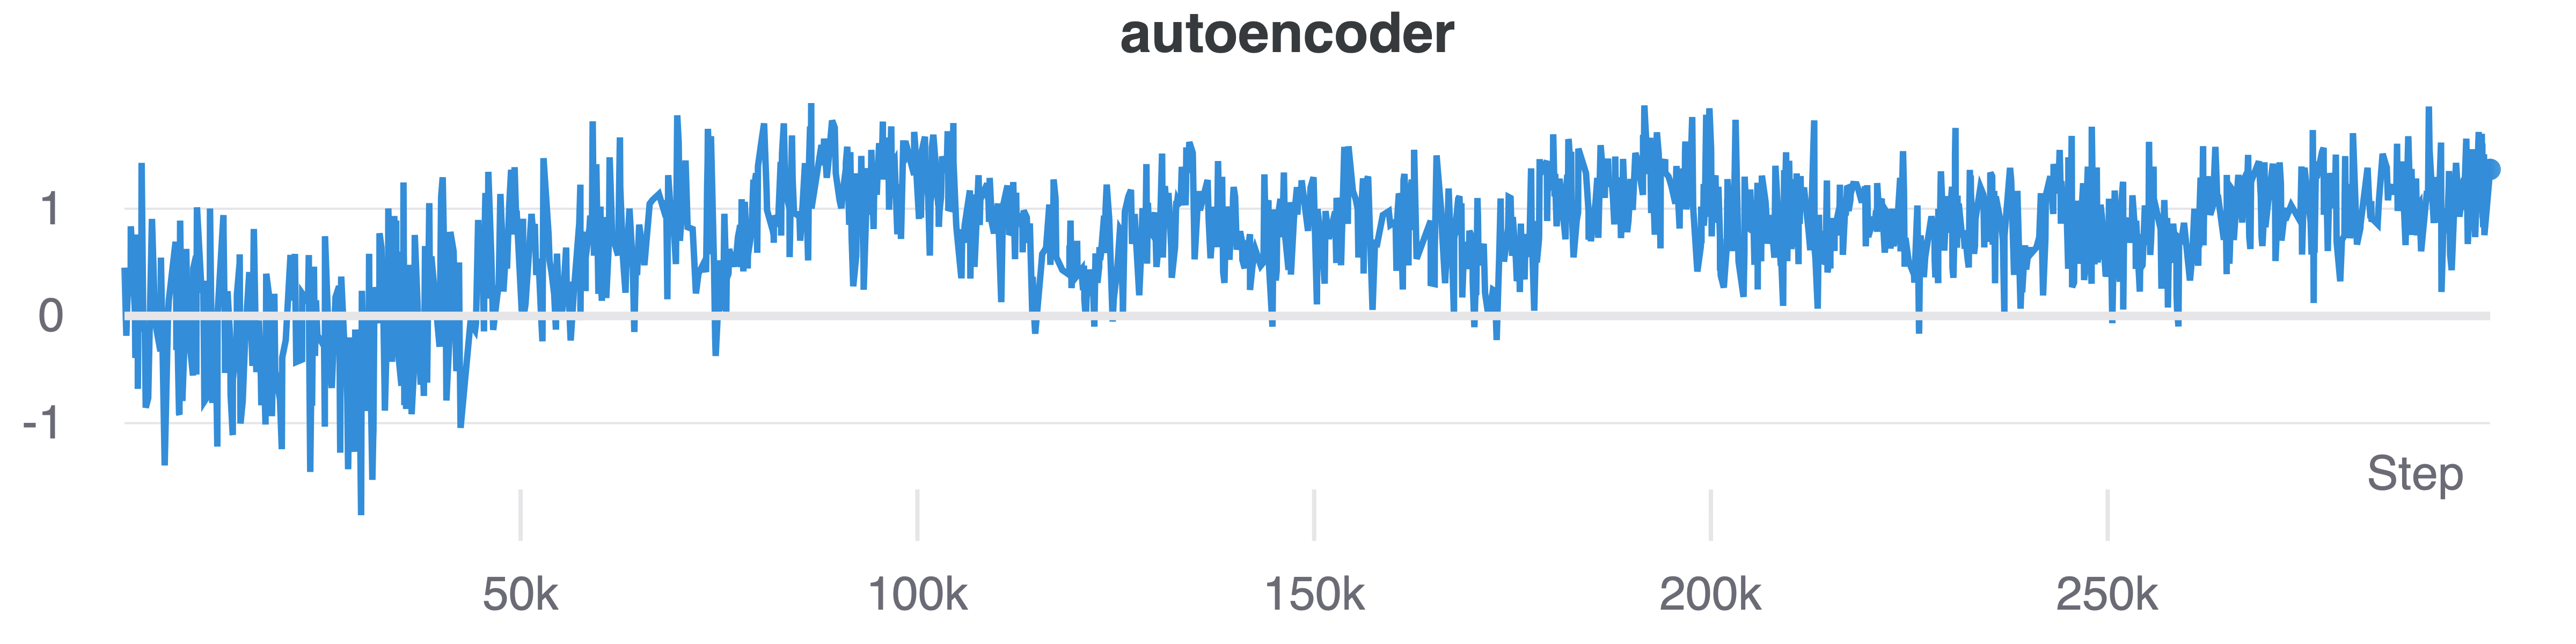
\includegraphics[width=\textwidth]{assets/figures/loss/a}
  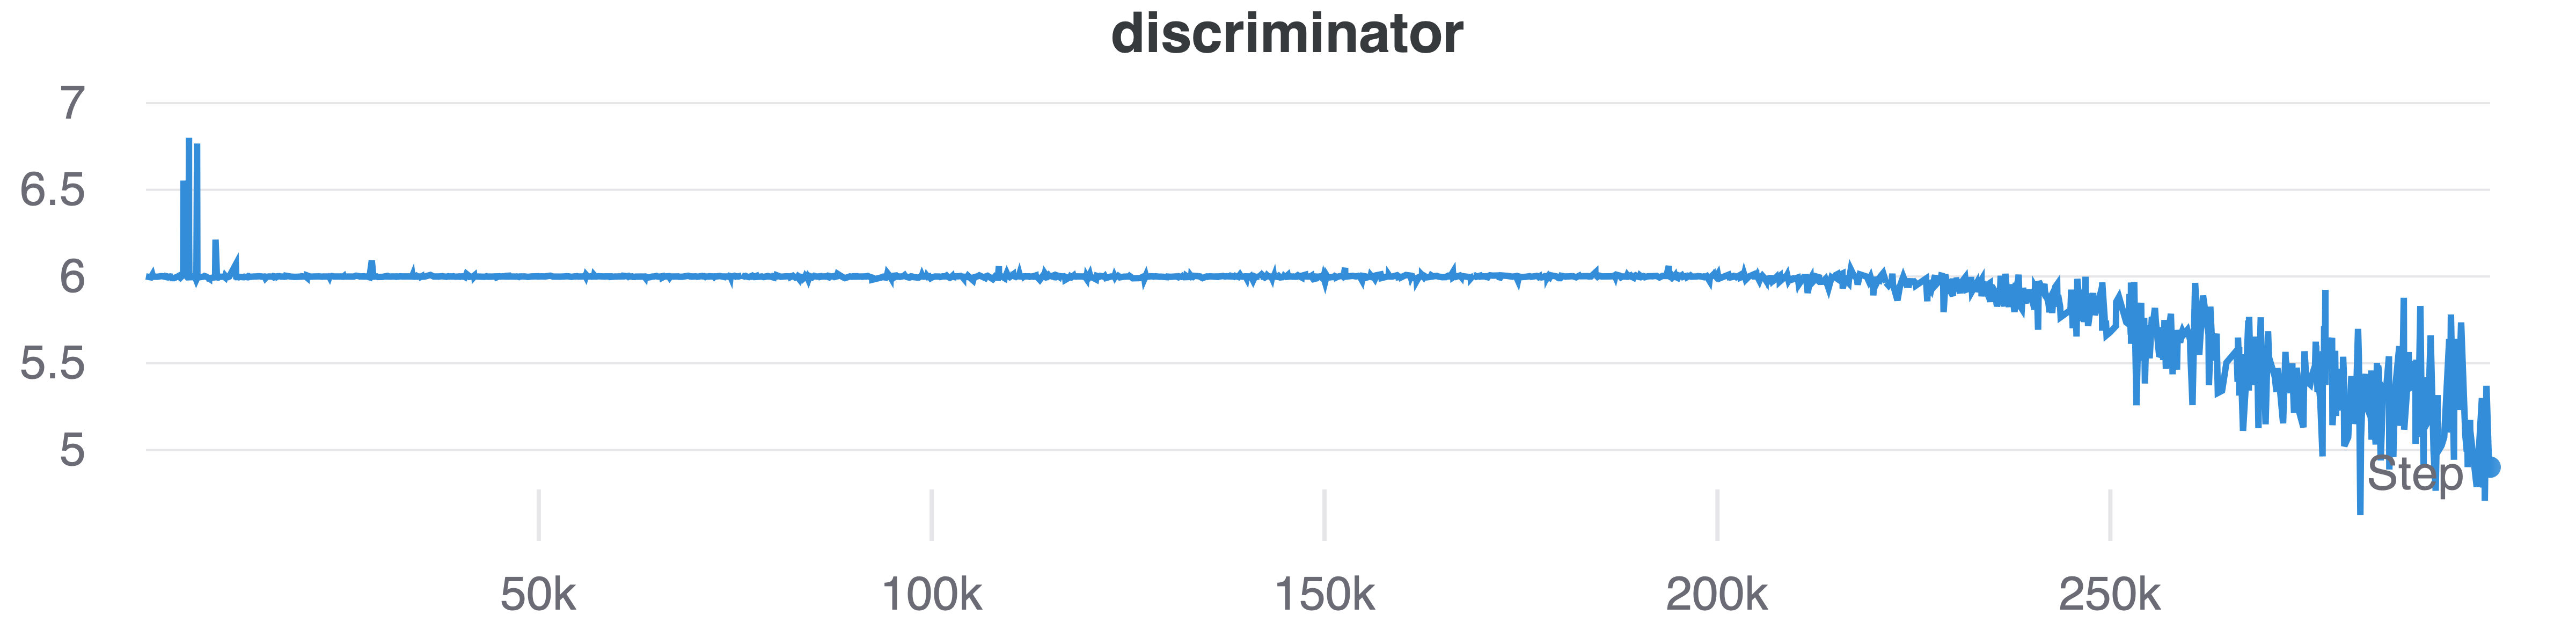
\includegraphics[width=\textwidth]{assets/figures/loss/d}
  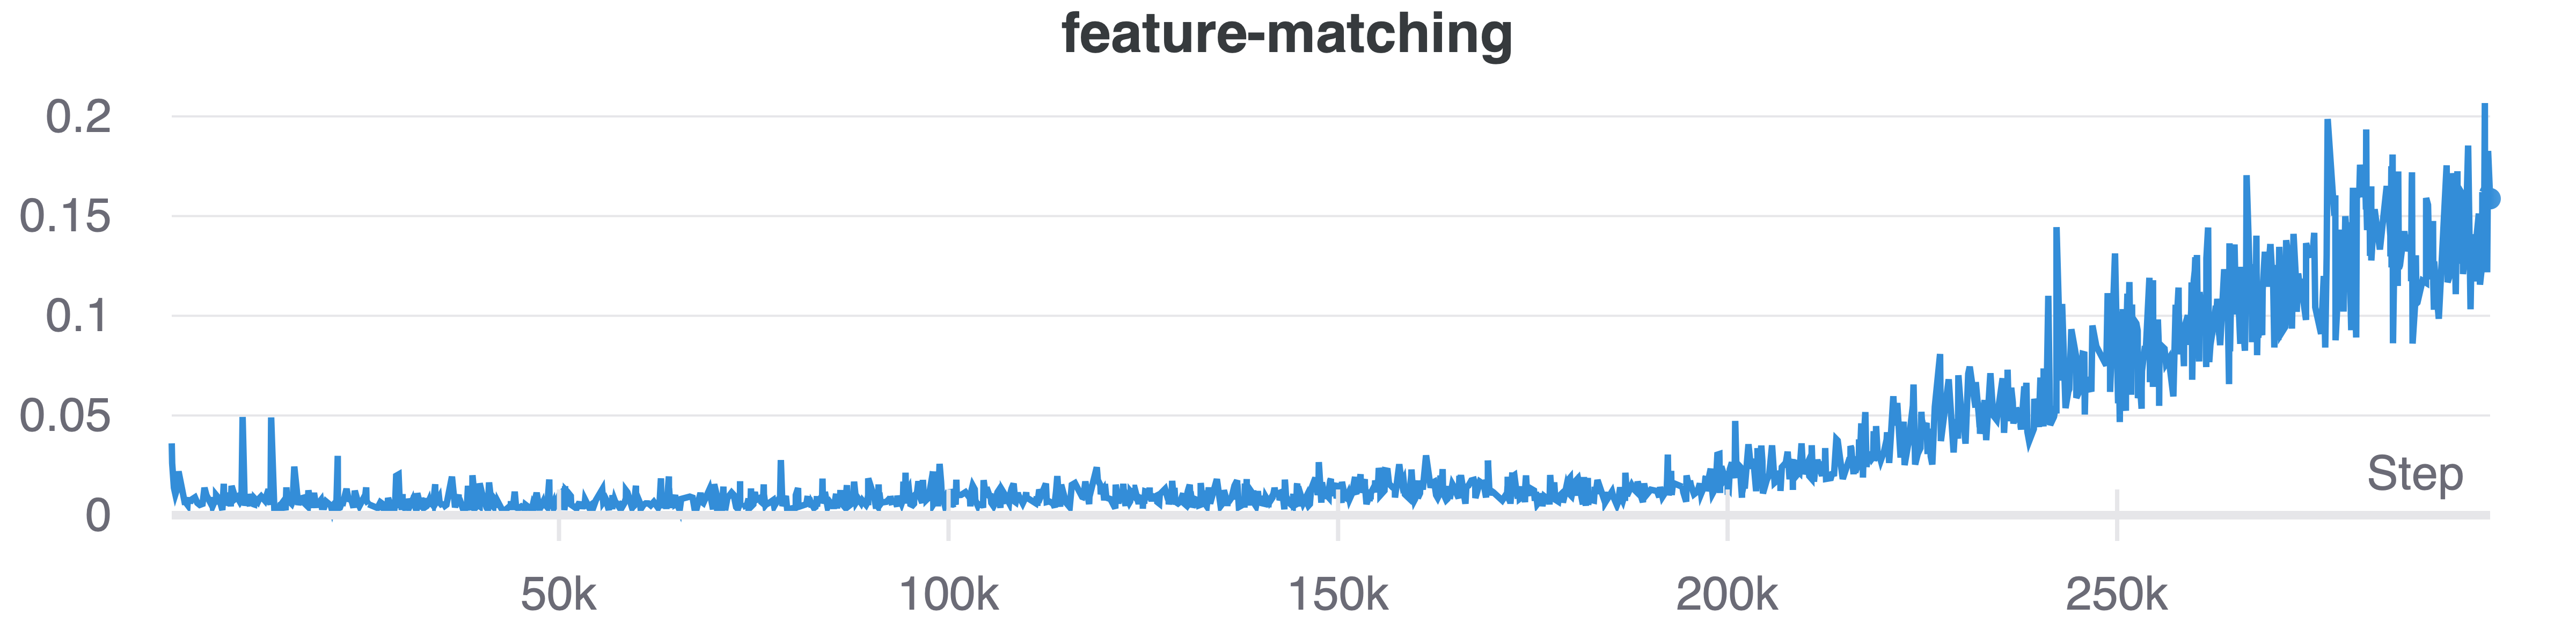
\includegraphics[width=\textwidth]{assets/figures/loss/fm}
  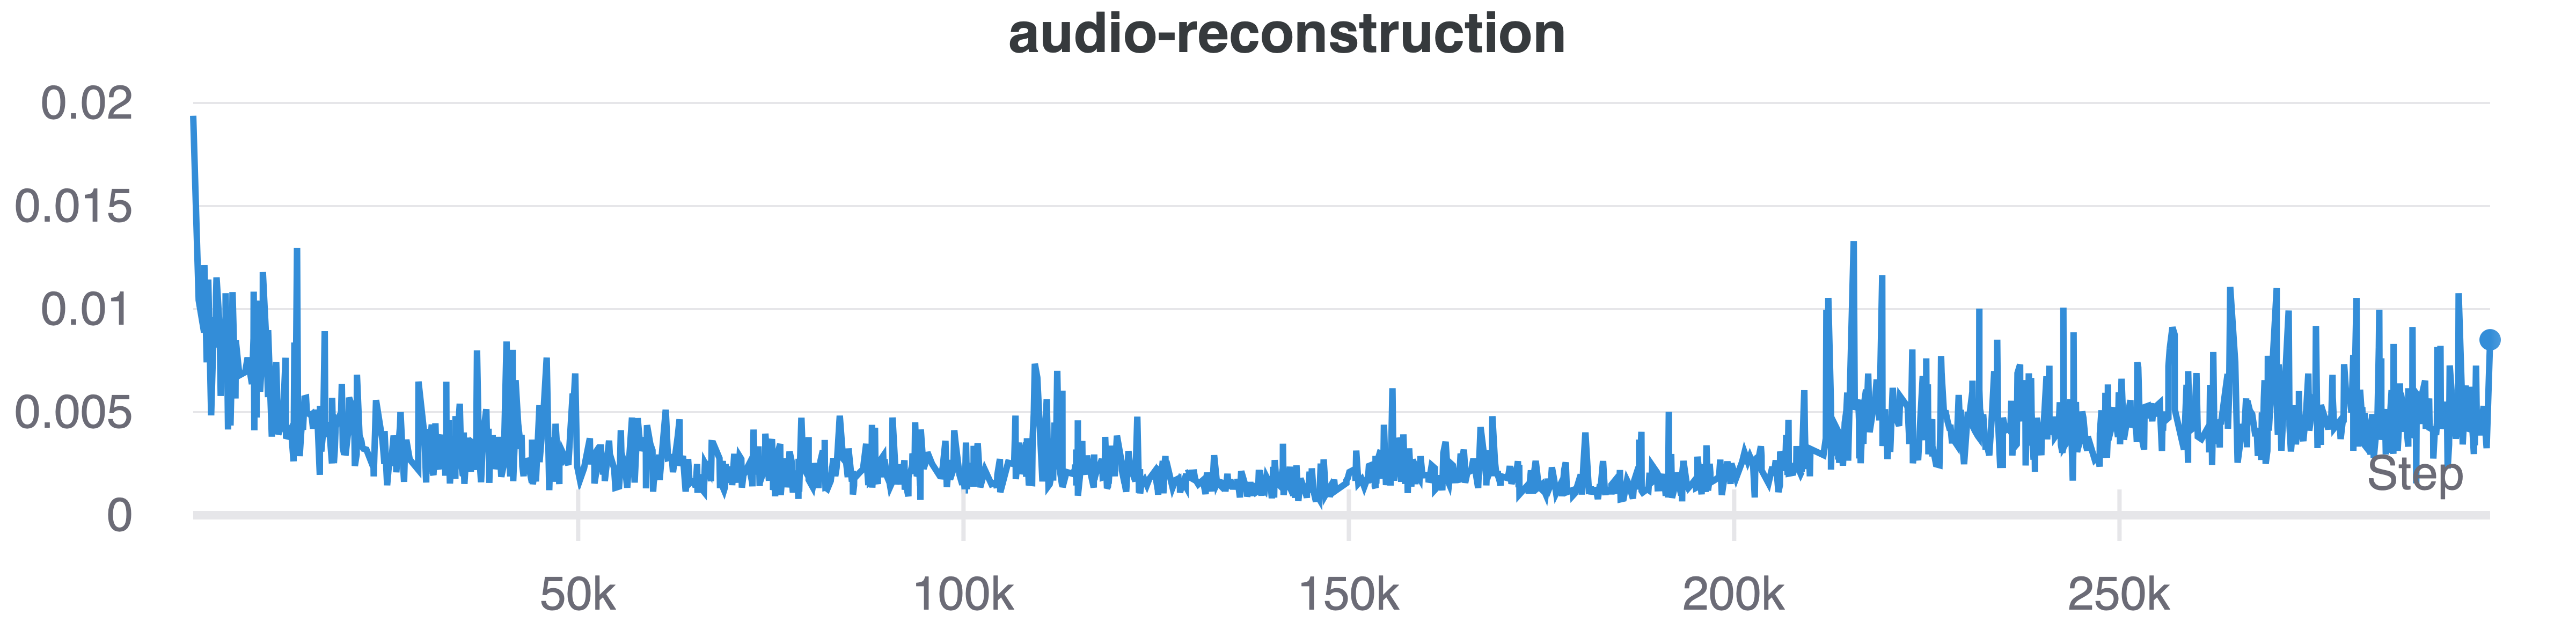
\includegraphics[width=\textwidth]{assets/figures/loss/ar}
  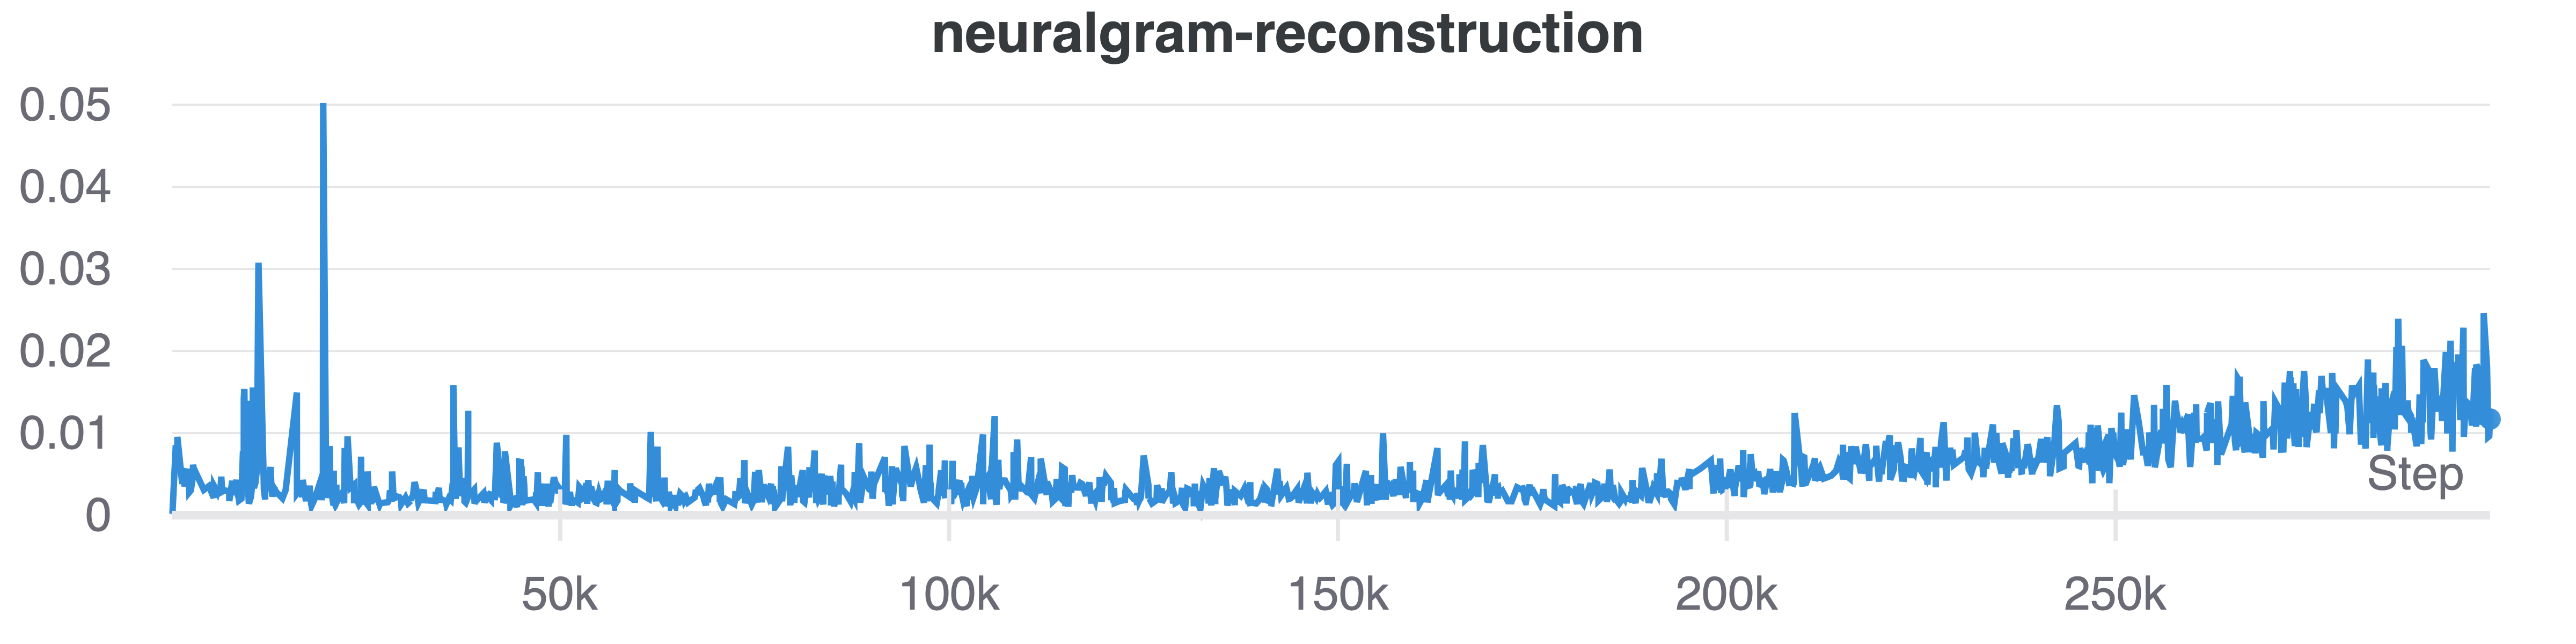
\includegraphics[width=\textwidth]{assets/figures/loss/nr}
\end{center}
\caption{A successful example of the training run. The audio quality keeps improving as long as the discriminator's loss fluctuates around 6.}
\label{fig:healthy-d}
\end{figure}

\end{appendices}

\end{document}
